\documentclass[tikz,border=10pt]{standalone}

\usepackage{tikz}
\usetikzlibrary{
  arrows.meta,
  backgrounds,
  calc,
  fit,
  positioning,
  shapes.geometric
}

\definecolor{inputblue}{RGB}{219,234,254}
\definecolor{processblue}{RGB}{224,242,254}
\definecolor{memorygreen}{RGB}{220,252,231}
\definecolor{rankpurple}{RGB}{237,233,254}
\definecolor{warnred}{RGB}{254,226,226}
\definecolor{evalorange}{RGB}{255,237,213}
\definecolor{groupblue}{RGB}{239,246,255}
\definecolor{groupgreen}{RGB}{240,253,244}
\definecolor{grouppurple}{RGB}{250,245,255}
\definecolor{grouporange}{RGB}{255,247,237}
\definecolor{linegray}{RGB}{71,85,105}
\definecolor{textgray}{RGB}{30,41,59}

\tikzset{
  font=\sffamily,
  >={Latex[length=2.4mm,width=1.8mm]},
  module/.style={
    rectangle,
    rounded corners=3pt,
    draw=#1!80!black,
    fill=#1,
    very thick,
    align=center,
    minimum width=33mm,
    minimum height=14mm,
    inner sep=5pt,
    text=textgray,
    font=\sffamily\small
  },
  smallmodule/.style={
    rectangle,
    rounded corners=3pt,
    draw=#1!80!black,
    fill=#1,
    thick,
    align=center,
    minimum width=32mm,
    minimum height=12mm,
    inner sep=4pt,
    text=textgray,
    font=\sffamily\footnotesize
  },
  store/.style={
    cylinder,
    shape border rotate=90,
    aspect=0.25,
    draw=#1!80!black,
    fill=#1,
    very thick,
    align=center,
    minimum width=32mm,
    minimum height=16mm,
    inner sep=4pt,
    text=textgray,
    font=\sffamily\footnotesize
  },
  decision/.style={
    diamond,
    draw=#1!80!black,
    fill=#1,
    very thick,
    align=center,
    aspect=2.2,
    inner sep=2pt,
    text=textgray,
    font=\sffamily\small
  },
  groupbox/.style={
    rectangle,
    rounded corners=7pt,
    draw=#1!75!black,
    fill=#1,
    very thick,
    inner sep=10pt
  },
  grouptitle/.style={
    rectangle,
    rounded corners=2pt,
    draw=#1!75!black,
    fill=white,
    thick,
    inner sep=2pt,
    font=\sffamily\bfseries\footnotesize,
    text=textgray
  },
  flow/.style={->, very thick, draw=linegray},
  dataflow/.style={->, thick, draw=linegray, dashed},
  feedback/.style={->, thick, draw=linegray, dotted},
  label/.style={font=\sffamily\footnotesize, text=textgray, fill=white, inner sep=1pt},
  subtitle/.style={font=\sffamily\scriptsize\itshape}
}

\begin{document}
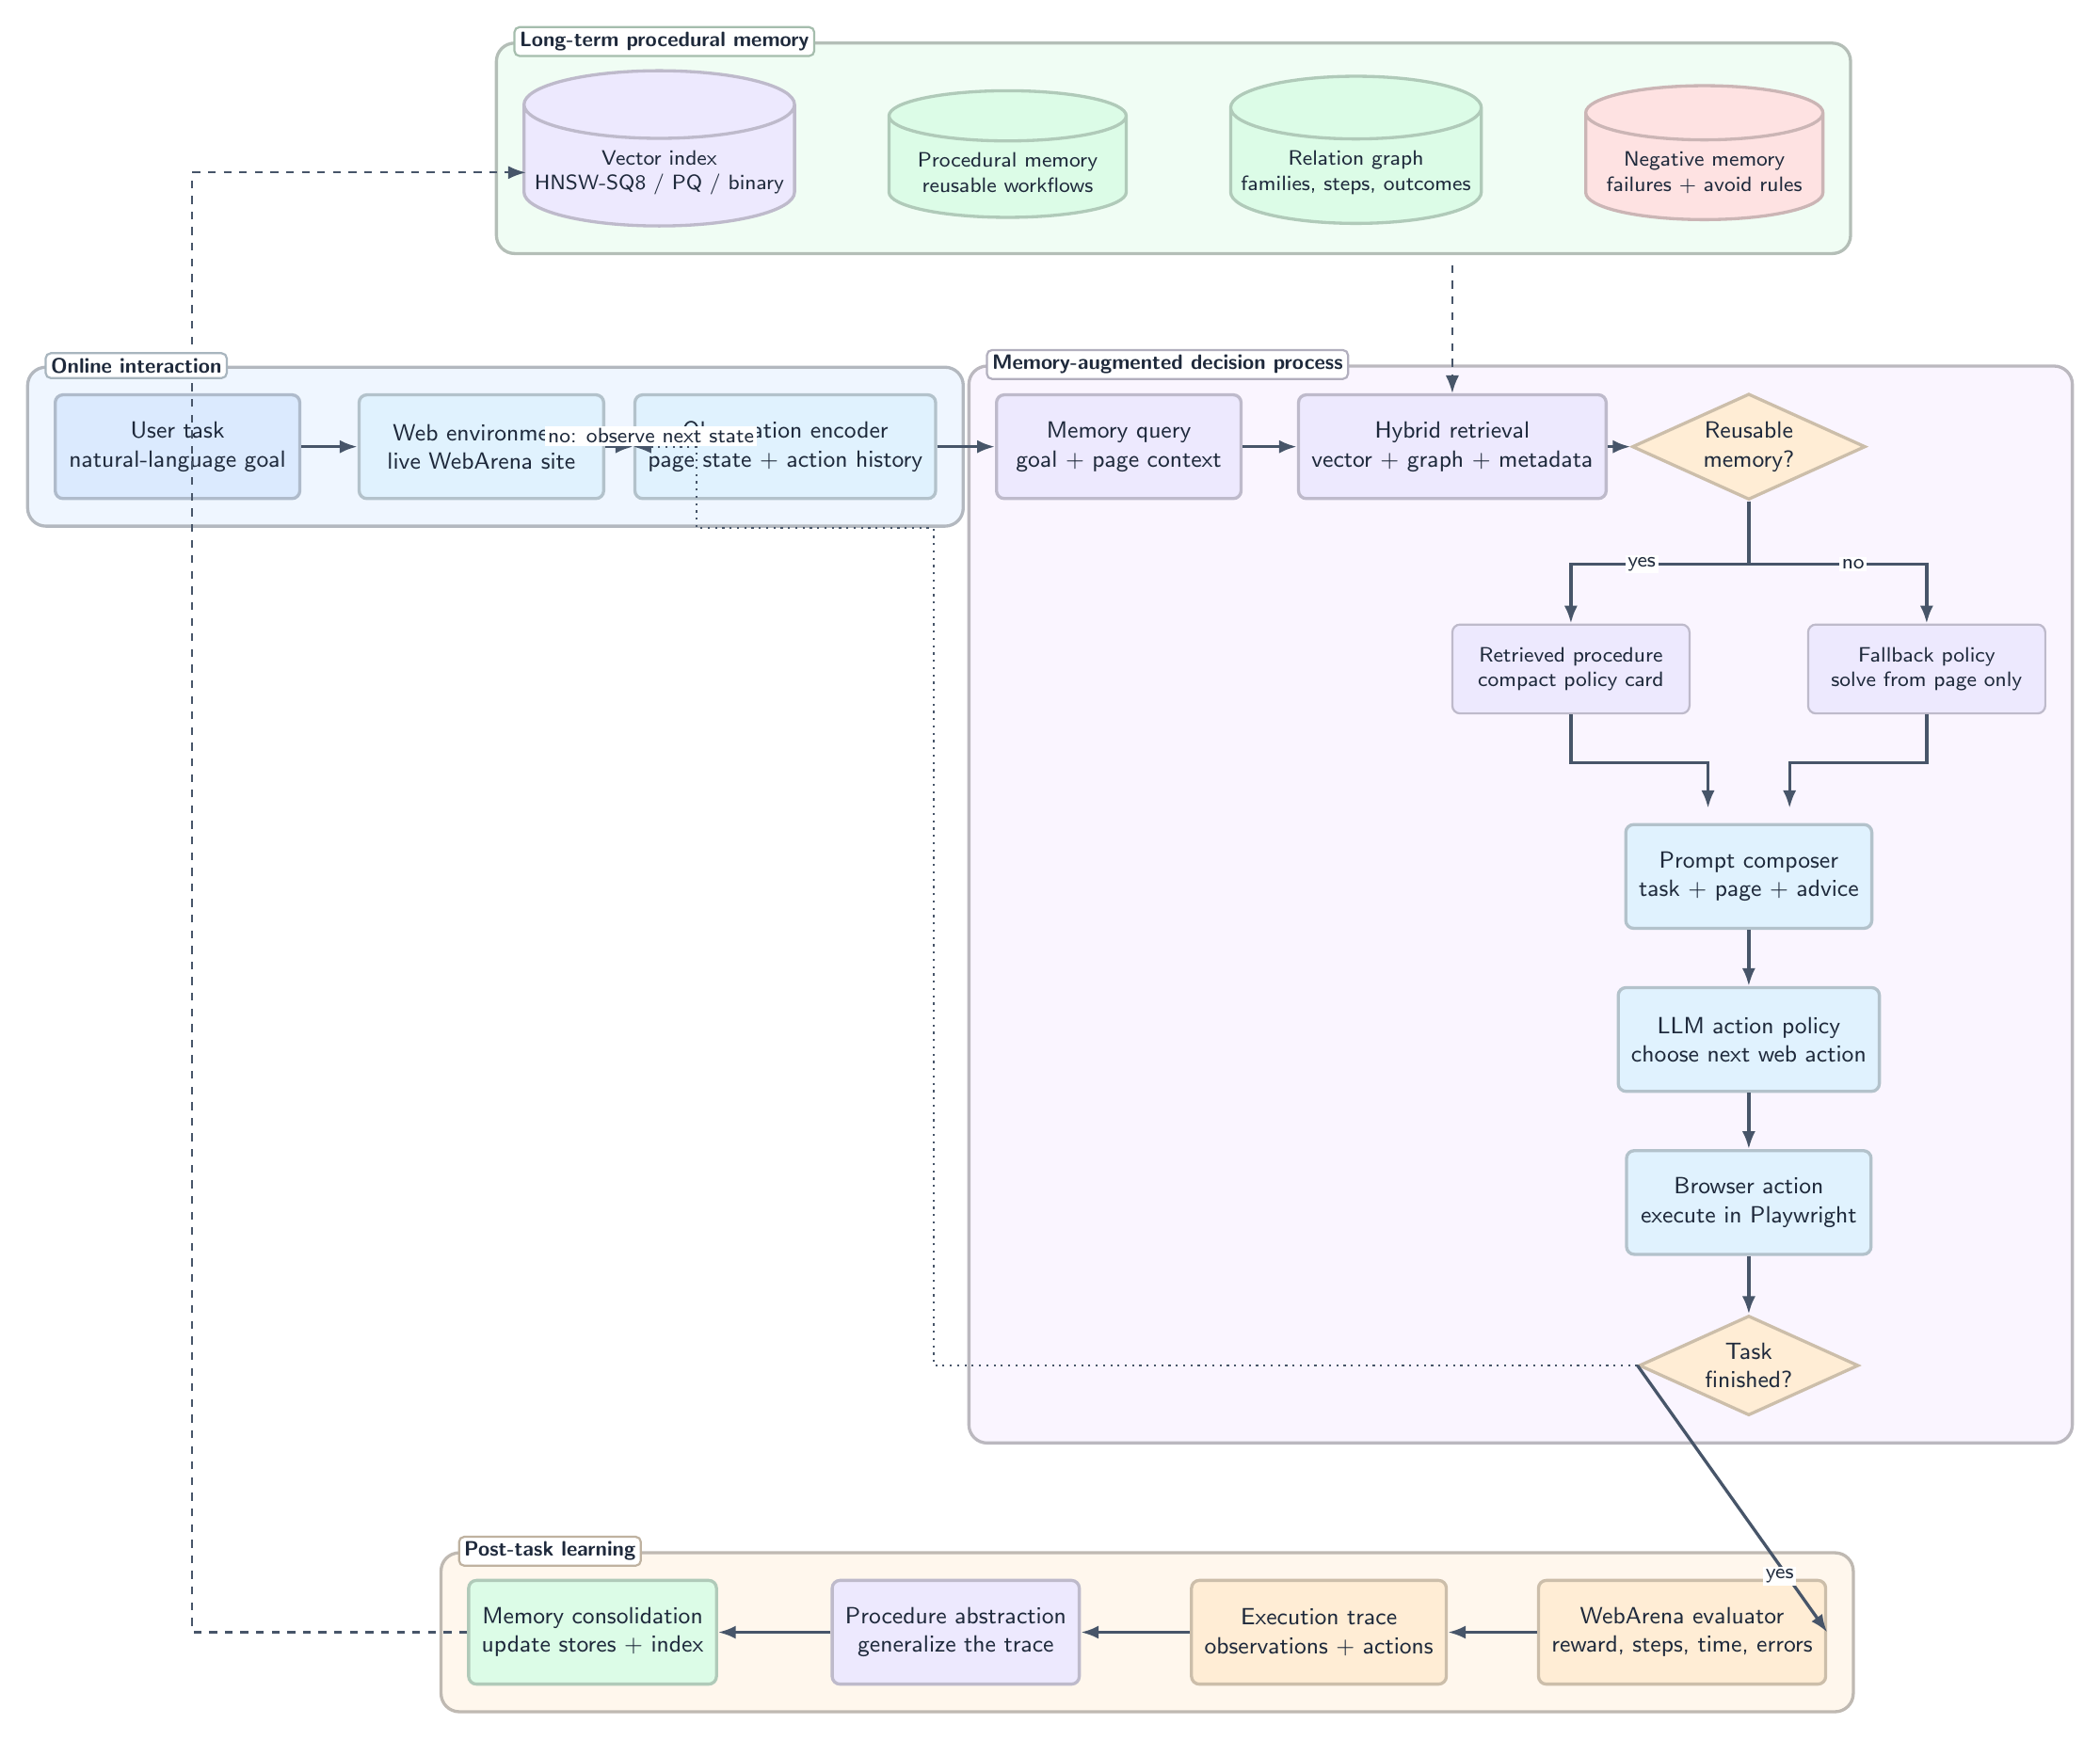
\begin{tikzpicture}[x=1cm,y=1cm]

% ---------------------------------------------------------------------
% Explicit coordinates give the figure research-paper spacing and keep arrows
% out of the main text boxes.
% ---------------------------------------------------------------------

% Long-term memory lane.
\node[store=rankpurple] (vecstore) at (6.5,3.7) {Vector index\\{\subtitle HNSW-SQ8 / PQ / binary}};
\node[store=memorygreen] (procstore) at (11.2,3.7) {Procedural memory\\{\subtitle reusable workflows}};
\node[store=memorygreen] (graphstore) at (15.9,3.7) {Relation graph\\{\subtitle families, steps, outcomes}};
\node[store=warnred] (negstore) at (20.6,3.7) {Negative memory\\{\subtitle failures + avoid rules}};

% Online interaction and retrieval lane.
\node[module=inputblue] (task) at (0,0) {User task\\{\subtitle natural-language goal}};
\node[module=processblue] (env) at (4.1,0) {Web environment\\{\subtitle live WebArena site}};
\node[module=processblue] (obs) at (8.2,0) {Observation encoder\\{\subtitle page state + action history}};
\node[module=rankpurple] (query) at (12.7,0) {Memory query\\{\subtitle goal + page context}};
\node[module=rankpurple] (retrieve) at (17.2,0) {Hybrid retrieval\\{\subtitle vector + graph + metadata}};
\node[decision=evalorange] (gate) at (21.2,0) {Reusable\\memory?};

% Policy and action lane.
\node[smallmodule=rankpurple] (memorycard) at (18.8,-3.0) {Retrieved procedure\\{\subtitle compact policy card}};
\node[smallmodule=rankpurple] (scratch) at (23.6,-3.0) {Fallback policy\\{\subtitle solve from page only}};
\node[module=processblue] (prompt) at (21.2,-5.8) {Prompt composer\\{\subtitle task + page + advice}};
\node[module=processblue] (llm) at (21.2,-8.0) {LLM action policy\\{\subtitle choose next web action}};
\node[module=processblue] (act) at (21.2,-10.2) {Browser action\\{\subtitle execute in Playwright}};
\node[decision=evalorange] (done) at (21.2,-12.4) {Task\\finished?};

% Post-task learning lane.
\node[module=memorygreen] (update) at (5.6,-16.0) {Memory consolidation\\{\subtitle update stores + index}};
\node[module=rankpurple] (abstract) at (10.5,-16.0) {Procedure abstraction\\{\subtitle generalize the trace}};
\node[module=evalorange] (trace) at (15.4,-16.0) {Execution trace\\{\subtitle observations + actions}};
\node[module=evalorange] (eval) at (20.3,-16.0) {WebArena evaluator\\{\subtitle reward, steps, time, errors}};

% ---------------------------------------------------------------------
% Main task flow.
% ---------------------------------------------------------------------
\draw[flow] (task) -- (env);
\draw[flow] (env) -- (obs);
\draw[flow] (obs) -- (query);
\draw[flow] (query) -- (retrieve);
\draw[flow] (retrieve) -- (gate);

% Memory decision routes. They are separated from the memory-store row.
\draw[flow] (gate.south) -- ++(0,-0.85) -| node[label, pos=0.25, left] {yes} (memorycard.north);
\draw[flow] (gate.south) -- ++(0,-0.85) -| node[label, pos=0.25, right] {no} (scratch.north);
\draw[flow] (memorycard.south) -- ++(0,-0.65) -| ($(prompt.north)+(-0.55,0.2)$);
\draw[flow] (scratch.south) -- ++(0,-0.65) -| ($(prompt.north)+(0.55,0.2)$);
\draw[flow] (prompt) -- (llm);
\draw[flow] (llm) -- (act);
\draw[flow] (act) -- (done);
\draw[flow] (done.west) -- node[label, near end, below] {yes} (eval.east);

% The within-task loop is routed through the empty corridor between observation
% and memory query, so it does not run over the decision boxes.
\coordinate (observeLoop) at (10.2,-12.4);
\draw[feedback]
  (done.west) -- (observeLoop) -- (10.2,-1.1) -- (7.0,-1.1) -- (7.0,0) -- node[label, pos=0.72, above] {no: observe next state} (obs.west);

% ---------------------------------------------------------------------
% Memory retrieval is shown as one group-level dependency. The individual
% stores are named inside the group; the retrieval module consumes the group.
% ---------------------------------------------------------------------
\draw[dataflow] (17.2,2.45) -- (retrieve.north);

% ---------------------------------------------------------------------
% Learning flow and memory updates. Update arrows leave from the left edge and
% rise outside the central decision process.
% ---------------------------------------------------------------------
\draw[flow] (eval) -- (trace);
\draw[flow] (trace) -- (abstract);
\draw[flow] (abstract) -- (update);

\coordinate (updateLoop) at (0.2,-16.0);
\draw[dataflow] (update.west) -- (updateLoop) |- (4.7,3.7);

% ---------------------------------------------------------------------
% Labeled group boxes.
% ---------------------------------------------------------------------
\begin{scope}[on background layer]
  \node[groupbox=groupgreen, fit=(vecstore)(procstore)(graphstore)(negstore)] (gmemory) {};
  \node[groupbox=groupblue, fit=(task)(env)(obs)] (gonline) {};
  \node[groupbox=grouppurple, fit=(query)(retrieve)(gate)(memorycard)(scratch)(prompt)(llm)(act)(done)] (gdecision) {};
  \node[groupbox=grouporange, fit=(update)(abstract)(trace)(eval)] (glearn) {};
\end{scope}

\node[grouptitle=memorygreen, anchor=west] at ($(gmemory.north west)+(0.25,0)$) {Long-term procedural memory};
\node[grouptitle=processblue, anchor=west] at ($(gonline.north west)+(0.25,0)$) {Online interaction};
\node[grouptitle=rankpurple, anchor=west] at ($(gdecision.north west)+(0.25,0)$) {Memory-augmented decision process};
\node[grouptitle=evalorange, anchor=west] at ($(glearn.north west)+(0.25,0)$) {Post-task learning};

\end{tikzpicture}
\end{document}
